% Analisi dei requisiti

\chapter{Analisi dei requisiti}\label{chap:requirements}

\section{Attori coinvolti}
Gli attori attivi nei vari scenari dei casi d'uso individuati sono quattro, di 
cui tre principali e uno secondario.
\subsection{Attori principali}
\subsubsection{Utente Zimbra}
L'applicazione è destinata solamente agli utenti Zimbra. Ciò si traduce nel 
fatto che si può accedere alle funzionalità di Teamwork solo se si è già in 
possesso di un'email Zimbra gestita dai loro server.  
\subsubsection{Utente OpenChat}
Un utente OpenChat, specializzazione dell'utente Zimbra, rappresenta un utente che utilizza un'istanza di Zimbra con la zimlet OpenChat installata. Questa zimlet permette di chattare con gli utenti Zimbra dello stesso server.

\subsubsection{Utente Teamwork web}
Un utente Teamwork web, specializzazione dell'utente OpenChat, rappresenta 
un utente che, oltre ad utilizzare un'istanza di Zimbra con la zimlet OpenChat, 
ha installato anche la zimlet Teamwork, applicazione di chat potenziata rispetto 
a OpenChat disponibile solo per la suite Zextras.

\subsection{Attori secondari}
\subsubsection{Server Zimbra}
Un server Zimbra è un'istanziazione della suite di prodotti Zimbra e, in caso, 
dei prodotti Zextras. Tramite esso si accede a tutti i dati del profilo Zimbra 
così da mantenerli sincronizzati tra le varie sessioni in uso.

\section{Casi d'uso principali}
Considerando l'obbiettivo del progetto (sez. \ref{sec:intaz}) e il metodo di 
lavoro utilizzato (sez. \ref{sec:pianificazione}), i casi d'uso (come i requisiti 
funzionali) sono stati sviluppati durante tutto il corso del progetto. 
In questa sezione vengono riportati e descritti i casi d'uso principali che 
sono stati delineati fin da subito tramite le richieste dell'azienda e quelli 
di alto livello, in modo da poter dare una visione d’insieme più precisa del 
prodotto sviluppato. \\

Ogni caso d'uso identificato viene qui riportato attraverso un codice univoco 
gerarchico nella forma:
$$ \textbf{UC \{codice\_padre\}.\{codice\_figlio\}  } $$
\begin{itemize}
	\item Le prime due lettere identificano che si tratta di un caso d'uso;
	\item Il codice padre è un numero univoco che identifica un caso d'uso;
	\item Il codice figlio è un numero progressivo che identifica i sottocasi;\\
\end{itemize}

\subsection{UCG - Caso d'uso generale}
\begin{figure}[H] 
	\centering
	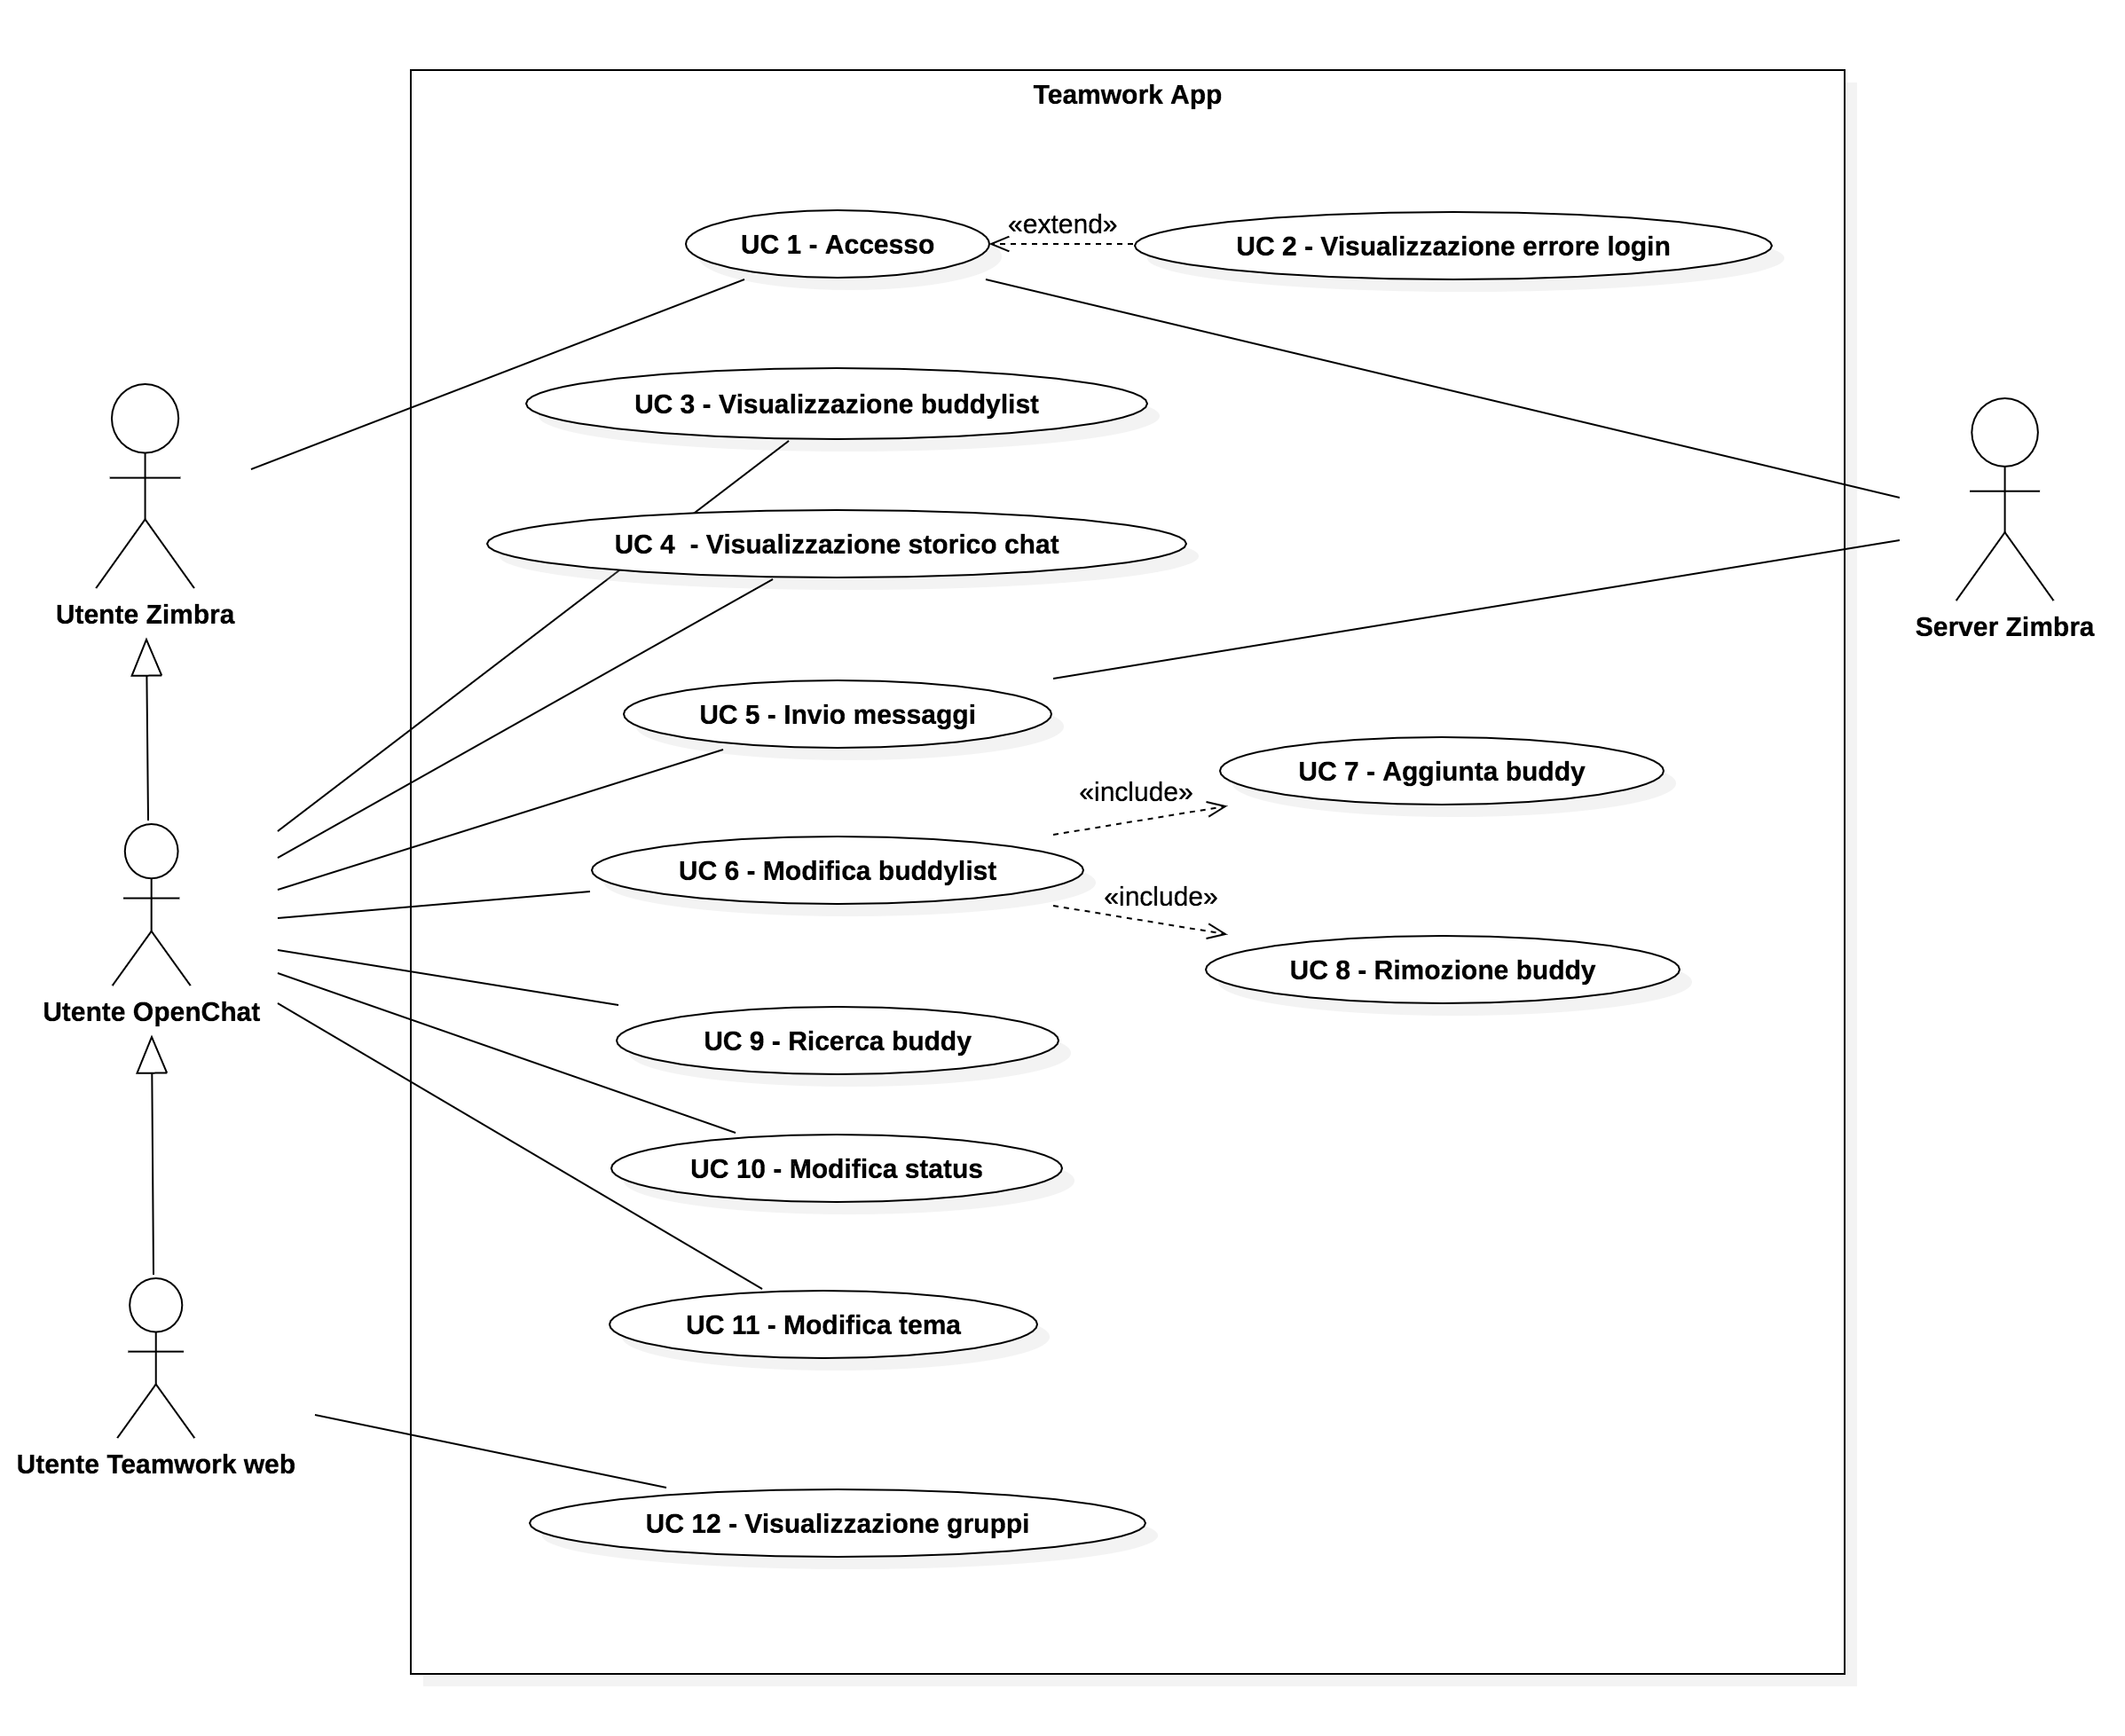
\includegraphics[scale=0.17]{UC/UCG}
	\caption{UCG - Caso d'uso generale}
\end{figure}
\usecase{Attore}{Desc}{pre}{post}{flusso}


\subsection{UC1 - Accesso}
\begin{figure}[H] 
	\centering
	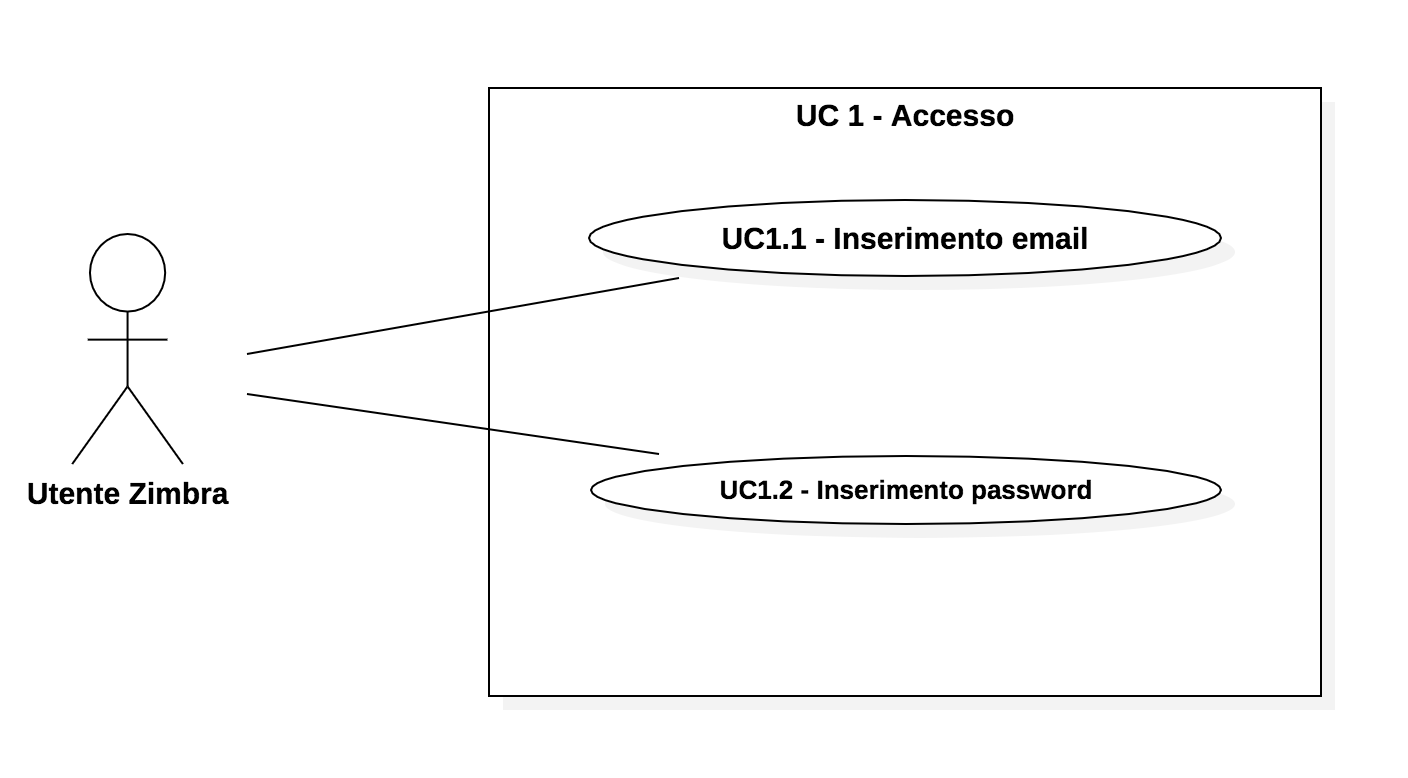
\includegraphics[scale=0.17]{UC/UC1}
	\caption{UC1 - Accesso}
\end{figure}
\usecase{Attore}{Desc}{pre}{post}{flusso}

\subsection{UC1.1 - Inserimento email}
\usecase{Attore}{Desc}{pre}{post}{flusso}
\subsection{UC1.2 - Inserimento password}
\usecase{Attore}{Desc}{pre}{post}{flusso}


\subsection{UC2 - Visualizzazione errore login}
\usecase{Attore}{Desc}{pre}{post}{flusso}


\subsection{UC3 - Visualizzazione buddylist}
\begin{figure}[H] 
	\centering
	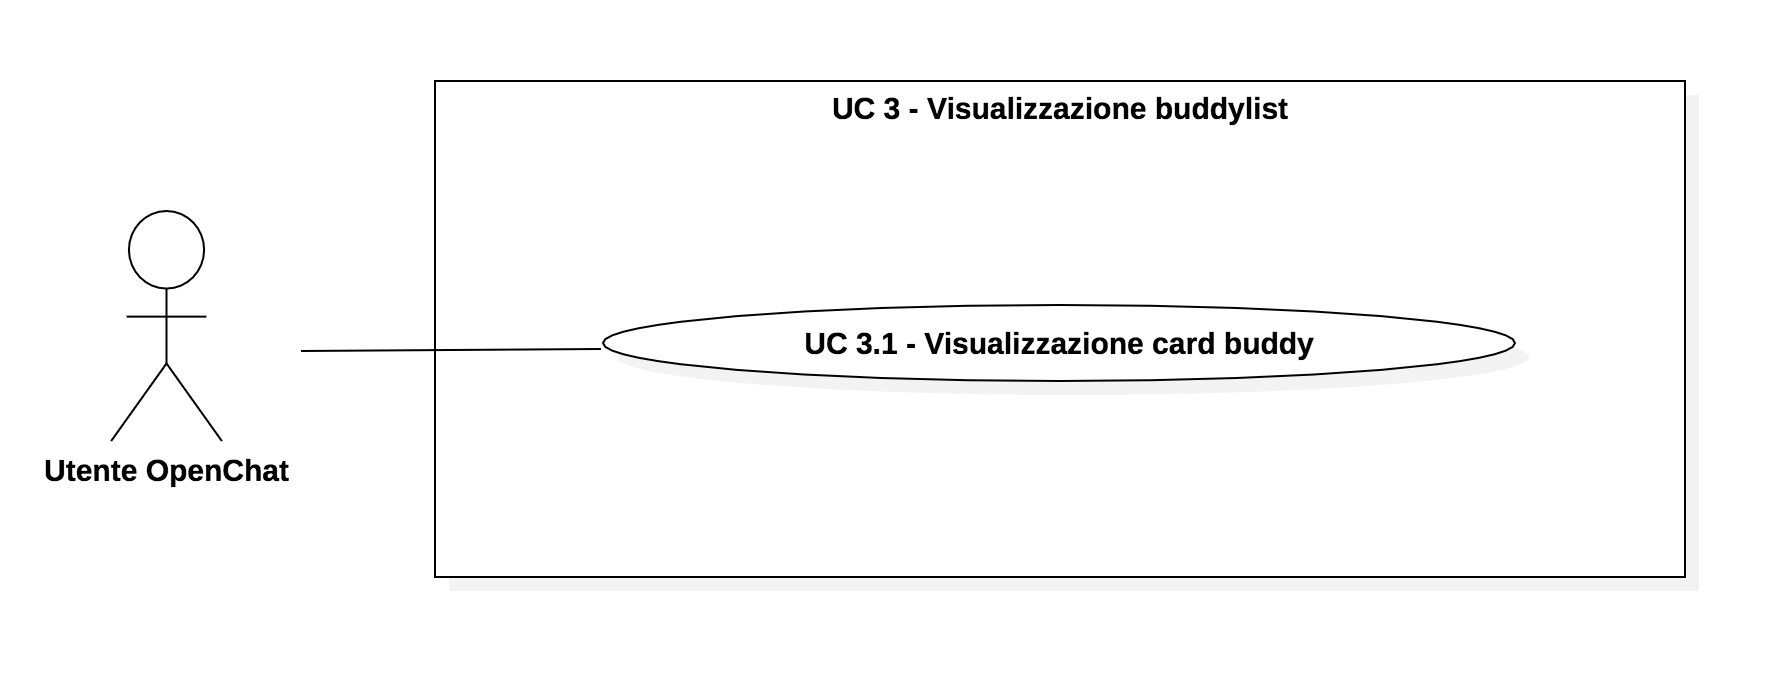
\includegraphics[scale=0.17]{UC/UC3}
	\caption{UC3 - Visualizzazione buddylist}
\end{figure}
\usecase{Attore}{Desc}{pre}{post}{flusso}

\subsection{UC3.1 - Visualizzazione card buddy}
\begin{figure}[H] 
	\centering
	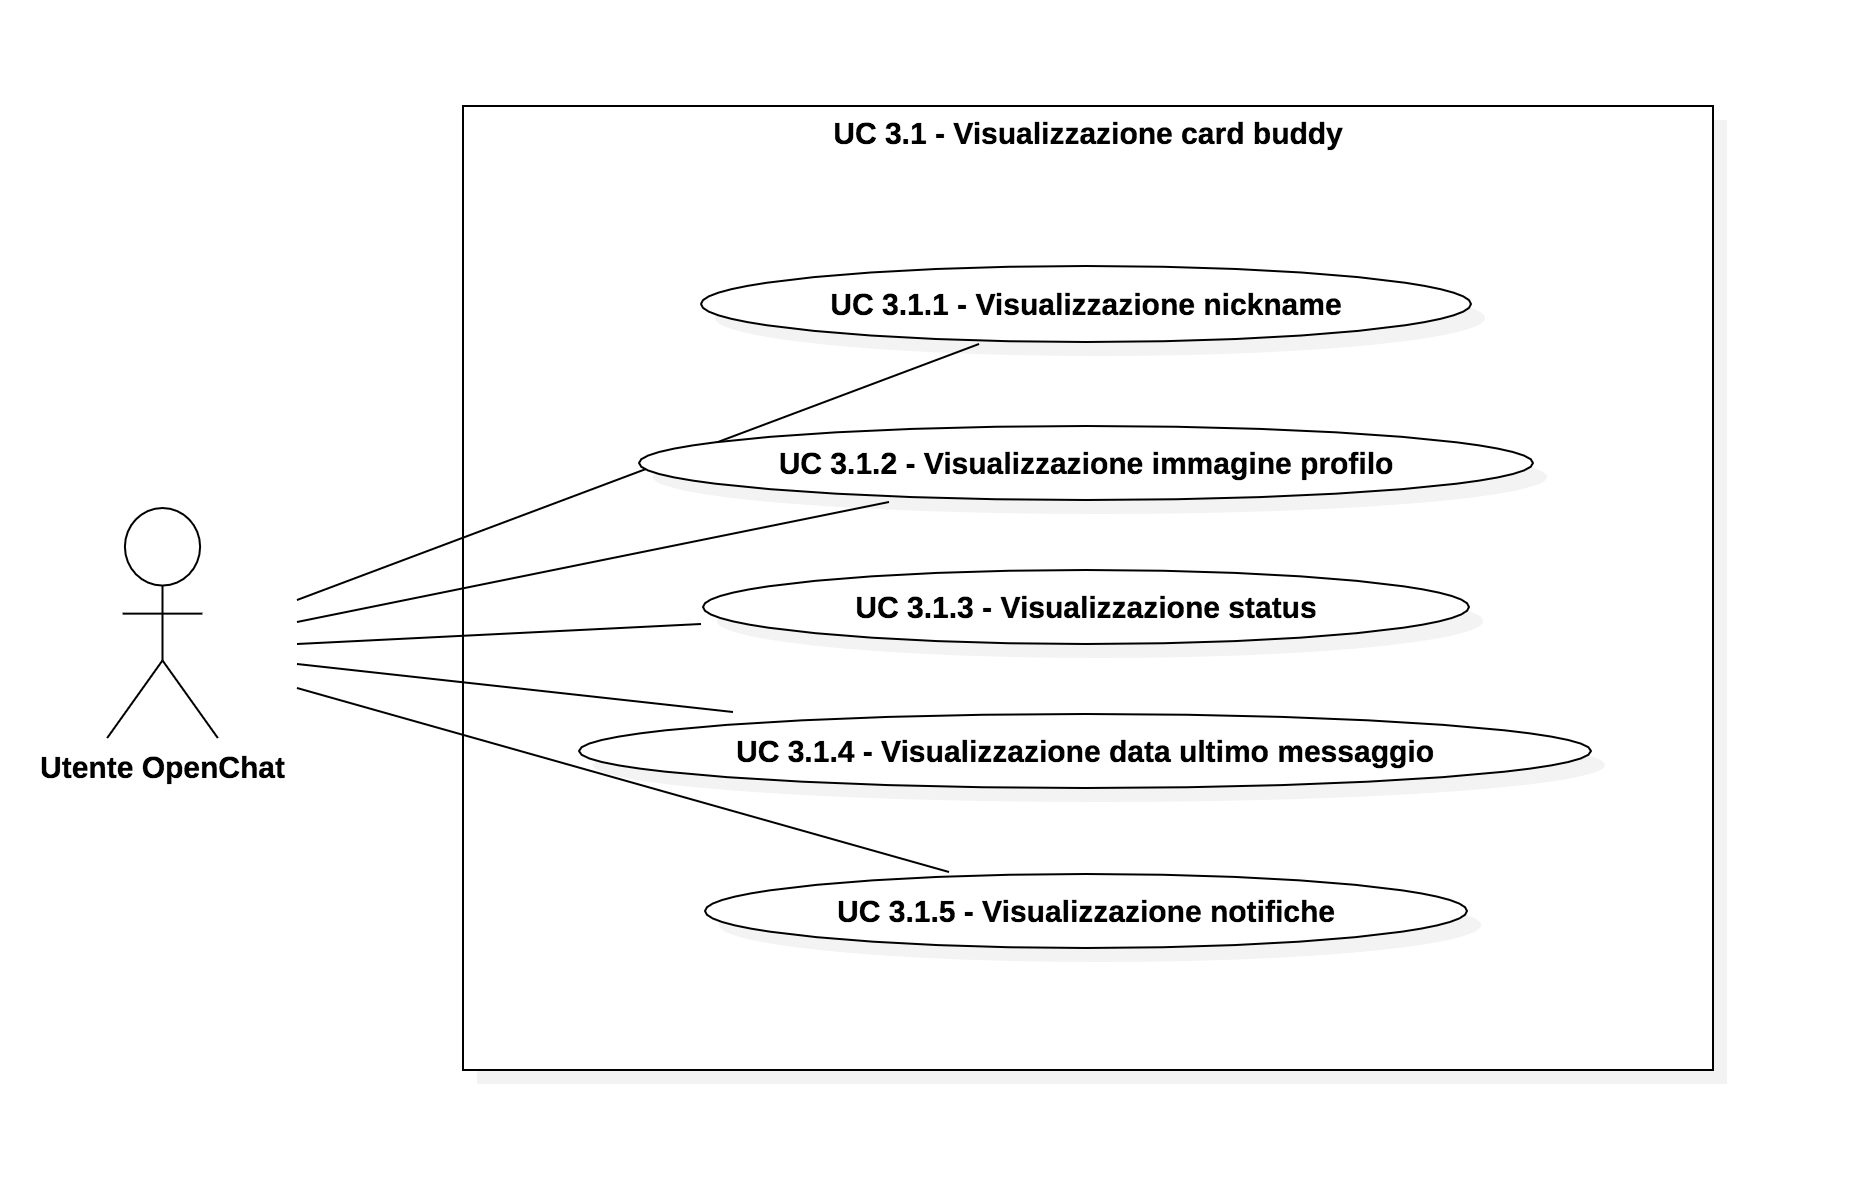
\includegraphics[scale=0.17]{UC/UC3_1}
	\caption{UC3.1 - Visualizzazione card buddy}
\end{figure}
\usecase{Attore}{Desc}{pre}{post}{flusso}

\subsection{UC3.1.1 - Visualizzazione nickname}
\usecase{Attore}{Desc}{pre}{post}{flusso}
\subsection{UC3.1.2 - Visualizzazione immagine profilo}
\usecase{Attore}{Desc}{pre}{post}{flusso}
\subsection{UC3.1.3 - Visualizzazione status}
\usecase{Attore}{Desc}{pre}{post}{flusso}
\subsection{UC3.1.4 - Visualizzazione data ultimo messaggio}
\usecase{Attore}{Desc}{pre}{post}{flusso}
\subsection{UC3.1.5 - Visualizzazione notifiche}
\usecase{Attore}{Desc}{pre}{post}{flusso}

\subsection{UC4 - Visualizzazione storico chat}
\begin{figure}[H] 
	\centering
	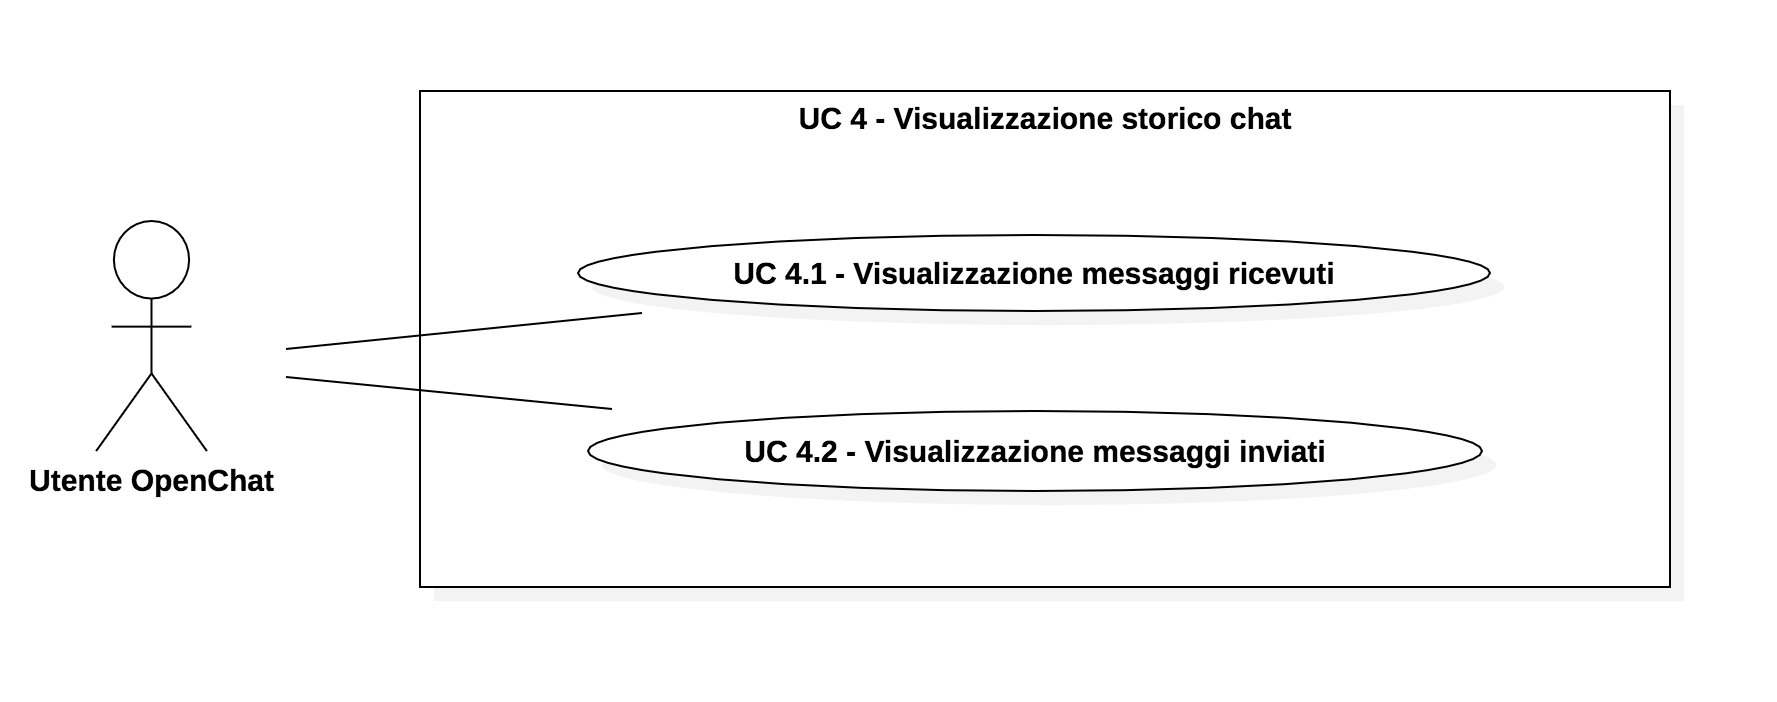
\includegraphics[scale=0.17]{UC/UC4}
	\caption{UC4 - Visualizzazione storico chat}
\end{figure}
\usecase{Attore}{Desc}{pre}{post}{flusso}

\subsection{UC4.1 - Visualizzazione messaggi ricevuti}
\usecase{Attore}{Desc}{pre}{post}{flusso}
\subsection{UC4.2 - Visualizzazione messaggi inviati}
\usecase{Attore}{Desc}{pre}{post}{flusso}

\subsection{UC5 - Invio messaggi}
\usecase{Attore}{Desc}{pre}{post}{flusso}
\subsection{UC6 - Modifica buddylist}
\usecase{Attore}{Desc}{pre}{post}{flusso}
\subsection{UC7 - Aggiunta buddy}
\usecase{Attore}{Desc}{pre}{post}{flusso}
\subsection{UC8 - Rimozione buddy}
\usecase{Attore}{Desc}{pre}{post}{flusso}
\subsection{UC9 - Ricerca buddy}
\usecase{Attore}{Desc}{pre}{post}{flusso}
\subsection{UC10 - Modifica status}
\usecase{Attore}{Desc}{pre}{post}{flusso}
\subsection{UC11 - Modifica tema}
\usecase{Attore}{Desc}{pre}{post}{flusso}
\subsection{UC12 - Visualizzazione gruppi}
\usecase{Attore}{Desc}{pre}{post}{flusso}


\section{Requisiti}
Ogni requisito qui riportato è identificato da un codice, ed è rappresentato nel seguente modo:
$$ \textbf{R \{importanza\}\{tipo\}\{numero\_vincolo\} } $$

\begin{itemize}
	\item "R" è prefisso di tutti i codici dei requisiti;
	\item Il primo valore rappresenta l'importanza: \textbf{0} se il requisito è obbligatorio, \textbf{1} se è desiderabile, \textbf{2} per gli opzionali;
	\item Il terzo valore indica il tipo: \textbf{F} per i requisiti funzionali, \textbf{Q} per quelli di qualità, \textbf{P} se prestazionale, \textbf{V} se di vincolo;
	\item L'ultimo numero indica il numero del vincolo. La struttura numerica di quest'ultimo rispetta le stesse regole dei Casi D'Uso.
\end{itemize}

\subsection{Principali requisiti funzionali}
\begin{longtable}{|c|c|}
	\hline
	\textbf{Id Requisito} & \textbf{Descrizione}\\
	\hline
	\endhead
	R0F1 & ....  \\ \hline 
	\caption{Requisiti di qualità}
	\label{tabella:req}
\end{longtable}

\subsection{Requisiti di vincolo}
\begin{longtable}{|c|c|}
	\hline
	\textbf{Id Requisito} & \textbf{Descrizione}\\
	\hline
	\endhead
	R0V1 & ....  \\ \hline 
	\caption{Requisiti di vincolo}
	\label{tabella:reqV}
\end{longtable}

\subsection{Requisiti di qualità}
\begin{longtable}{|c|c|}
	\hline
	\textbf{Id Requisito} & \textbf{Descrizione}\\
	\hline
	\endhead
	R0Q1 & ....  \\ \hline 
	\caption{Requisiti di qualità}
	\label{tabella:reqQ}
\end{longtable}

